\documentclass{article} % For LaTeX2e
\usepackage{nips13submit_e,times}
\usepackage{hyperref}
\usepackage{url}
\usepackage{verbatim}
\usepackage{graphicx}
\usepackage{subcaption}
\usepackage{listings}
%\documentstyle[nips13submit_09,times,art10]{article} % For LaTeX 2.09


\title{Learning Programs through Bayesian Inference and Planning}

\begin{comment}
\author{
David S.~Hippocampus\thanks{ Use footnote for providing further information
about author (webpage, alternative address)---\emph{not} for acknowledging
funding agencies.} \\
Department of Computer Science\\
Cranberry-Lemon University\\
Pittsburgh, PA 15213 \\
\texttt{hippo@cs.cranberry-lemon.edu} \\
\And
Coauthor \\
Affiliation \\
Address \\
\texttt{email} \\
\AND
Coauthor \\
Affiliation \\
Address \\
\texttt{email} \\
\And
Coauthor \\
Affiliation \\
Address \\
\texttt{email} \\
\And
Coauthor \\
Affiliation \\
Address \\
\texttt{email} \\
(if needed)\\
}
\end{comment}
% The \author macro works with any number of authors. There are two commands
% used to separate the names and addresses of multiple authors: \And and \AND.
%
% Using \And between authors leaves it to \LaTeX{} to determine where to break
% the lines. Using \AND forces a linebreak at that point. So, if \LaTeX{}
% puts 3 of 4 authors names on the first line, and the last on the second
% line, try using \AND instead of \And before the third author name.

\newcommand{\fix}{\marginpar{FIX}}
\newcommand{\new}{\marginpar{NEW}}

%\nipsfinalcopy % Uncomment for camera-ready version

\begin{document}


\maketitle

\begin{abstract}
How can machine learning techniques be used to solve problems whose solutions are best represented as computer programs? For example, suppose a researcher wants to design a probabilistic graphical model for a novel domain. Searching the space of probabilistic models automatically is notoriously difficult and is especially difficult when the latent variables are possible. However, when researchers seem able to relatively easily adapt commonly used modeling motifs to new domains. In doing so, they draw on abstractions such as trees, chains, grids and plates to constrain and direct the kinds of models they produce. This suggests that before we ask machine learning algorithms to discover parsimonious models of new domains, we should develop techniques that enable our algorithms to automatically learn these ``graphical conepts'' in much the same way that researchers themselves do, by seeing examples in the literature. One natural way to think of these graphical concepts is as programs that take sets of random variables and produce graphical models that relate them. In this work, we describe the SEC algorithm, which attempts to learn a distribution over programs by incrementally finding program components that commonly help to solve problems in a given domain, and we show prelimarily that SEC is able to discover the graphical concepts that underlie many of the common graphical model structures.  
\end{abstract}


\section{Introduction}

The vast majority of research in machine learning is focused on utilizing large amounts of noisy data living in high-dimensional, real-valued vector spaces. Such research has been immensely successful and has enabled automatic and accurate modelling on a scale that was previously infeasible. However, when we want to build a car, draw a painting, or design the machine learning models to which we apply our new algorithms and techniques, we face problems that current machine learning tools are unable to handle. The highly structured objects that humans produce seems to require a different representation than the ones which machine learning algorithms have most successfully employed. 

To address this problem, many structured representations have been proposed in the machine learning and AI literatures: learning over graphs \cite{}, grammars\cite{}, Horn clauses\cite{}, relations{}, etc., has been investigated. These are representations that attempt to bridge the gap between the tractablity of learning and reasoning in smooth continuous spaces and the expressivity of general purpose programming languages. 

However, many of the most natural representations of structured domains are best described as programs and are difficult to fit into more restrictive representations.  To take an example directly from the machine learning literature, consider the plate notation~\cite{DBLP:journals/jair/Buntine94} commonly used to describe graphical models over collections of variables. A typical example is shown in Figure~\ref{fig:lda_plate}~\cite{DBLP:journals/jmlr/BleiNJ03}. The goal of plate notation is precisely to express the notion of a ``for loop'' within the graphical model representation. One reason this is a convenient tool is that researchers conceptualize their models as sampling procedures -- easily expressed as programs (see Figure~\ref{fig:lda_code}, but not as static graphs -- and can use plate notation to express a commonly occuring control structure. In fact, the field of probabilistic programming, which has gained recent popularity, is spurred on by exactly the motivation that our models are most naturally expressed as programs. 

Suppose, then, that we want to create machine learning algorithms that can help discover good models for data in novel domains; that is, we want algorithms that discovers the structure of the latent graphical model underlying the data. This is a field of active research \ 

In this paper, we describe our approach to learning over structured representations as a search over the space of programs in a functional programming language. We characterize learning in this space as incrementally developing a weighted library of program abstractions, i.e. a collection of subroutines, that are commonly used to solve problems in a given domain. The SEC algorithm (for Sequential Exploration-Compression), which we present here, takes a set of related tasks and produces a distribution over programs that solve those tasks; as it refines this distribution, SEC is able to search the space of programs more efficiently and solve more tasks. 

We will present here two domains of interest. First, continuing with the example above, we will describe how SEC can learn to efficiently explore the space of relevant graphical models for a given problem. Second, we will examine SEC's performance on a completely different type of task, in which we want to an algorithm to build tall and physically stable block towers. 

\lstset{
	basicstyle=\scriptsize\ttfamily,
    commentstyle=\color{white!40!black},
    escapechar=+,
    escapebegin=\color{white!40!black},
    escapeend={},
    keywordstyle=\bfseries\color{Periwinkle},
    numbers=left,
    numberstyle=\sffamily\tiny\color{gray},
}


\begin{figure}[h]
\centering
\begin{subfigure}{.5\textwidth}
  \centering
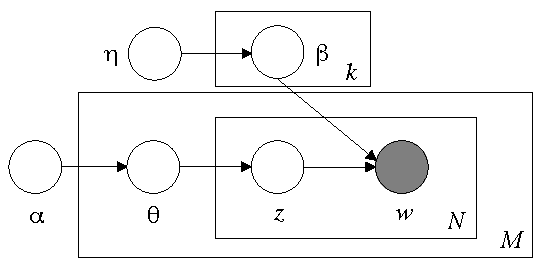
\includegraphics[width=.7\linewidth]{./figures/lda_plate_blei.pdf}
  \caption{An example of a typical plate notation use. \label{fig:lda_plate}}

\end{subfigure}%
\begin{subfigure}{.4\textwidth}
	\begin{lstlisting}[frame=single, numbers=none, xleftmargin=0pt]
	for +$k$+ = 1:NumTopics
	  +$\beta$+[k] +$\sim$+ Dirichlet(+$\eta$+)
	for m = 1:NumDocuments
	  +$\theta$+[m] +$\sim$+ Dirichlet(+$\alpha$+) 
	  for n = 1:NumWords 
	    z +$\sim$+ Categorical(+$\theta$+[m])
	    w+$\sim$+ Categorical(+$\beta$+[z])
	\end{lstlisting}
  \caption{The same model as a program.}
  \label{fig:lda_code}
\end{subfigure}
\caption{The popular Latent Dirichlet Allocation model in two forms.}
\label{fig:lda}
\end{figure}


Here, we present an approach to learning 

Motivation: Many approaches to constructive machine learning use structured representations, such as graphs, grammars, Horn clauses, relations, ..., ???. All of these may be thought of as a program - programs are at least as expressive as these other representations.

% TODO: Sequential EC? SEC? What is a good name for this?
The space of programs is enormous and inherently unpredictable \cite{PACunpredictability}.
We introduce a new algorithm, SEC, for searching the space of programs.
Two main ideas underly SEC:
\begin{itemize}
\item \emph{Learning to search}: Programs admit compositionality and reuse of subprograms. SEC exploits this compositionality to learn a library of program fragments, which it then reuses when performing further searches for programs.
In a multitask setting, this permits bootstrap learning of more complicated programs after the synthesis of simpler programs.
\item \emph{Incremental Program Synthesis}: In many search problems, there is a natural means of assigning partial credit for partially-correct solutions. SEC uses this partial credit to select promising programs and modify them, creating complicated programs step-by-step.
Rather than using a mutation operator, as in genetic programming, or Metropolis-Hastings proposals, as in \cite{MHprogramInduction}, SEC uses function composition to combine smaller programs in to larger ones.
\end{itemize}

The SEC algorithm comes from a generative model over compositions of functions drawn from a stochastic grammar over programs.
We describe this model, as well as how we perform inference, in ...

SEC treats planning as an inference problem.

\section{The SEC Algorithm}
\subsection{Generative Model}
\subsection{Inference}
\subsection{Program Representation}

\section{Application to Graphical Model Structure Learning}

Learning the structure of graphical models that capture the independencies underlying a dataset is an active area of research\cite{adams-wallach-ghahramani-2010a}\cite{ISI:000240797500002}\cite{ISI:000178037200004}\cite{ISI:A1995RX35400001}. Graphical model structures enforce the conditional independences a modeler believes exists among latent and observed random variables\cite{DBLP:books/daglib/0066829}. 

\subsection{Graph Combinators}

\subsection{Learning Graphical Models}

\begin{figure}
\begin{minipage}[c][8cm][t]{.4\textwidth}
  \vspace*{\fill}
  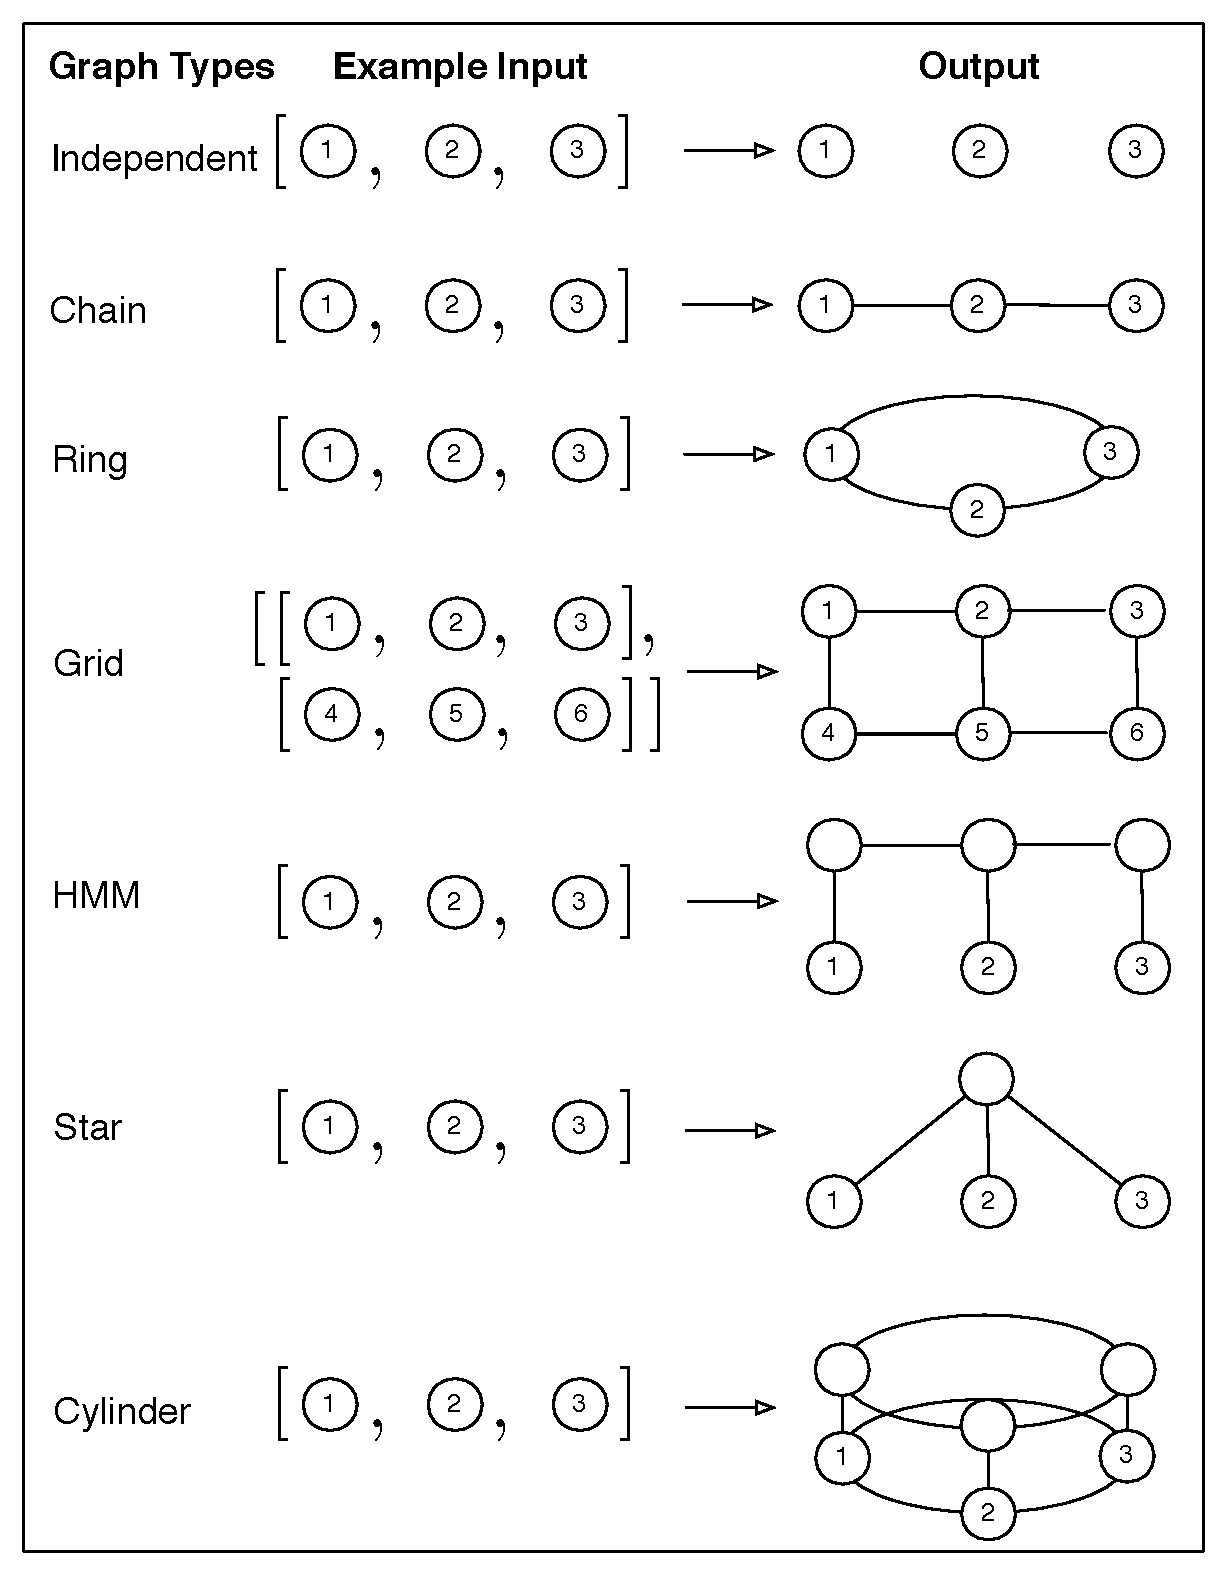
\includegraphics[width=\linewidth]{./figures/tasks.pdf}
  \caption{test figure one}
  \label{fig:test1}
\end{minipage}%
\begin{minipage}[c][8cm][t]{.3\textwidth}
  \vspace*{\fill}
  \fbox{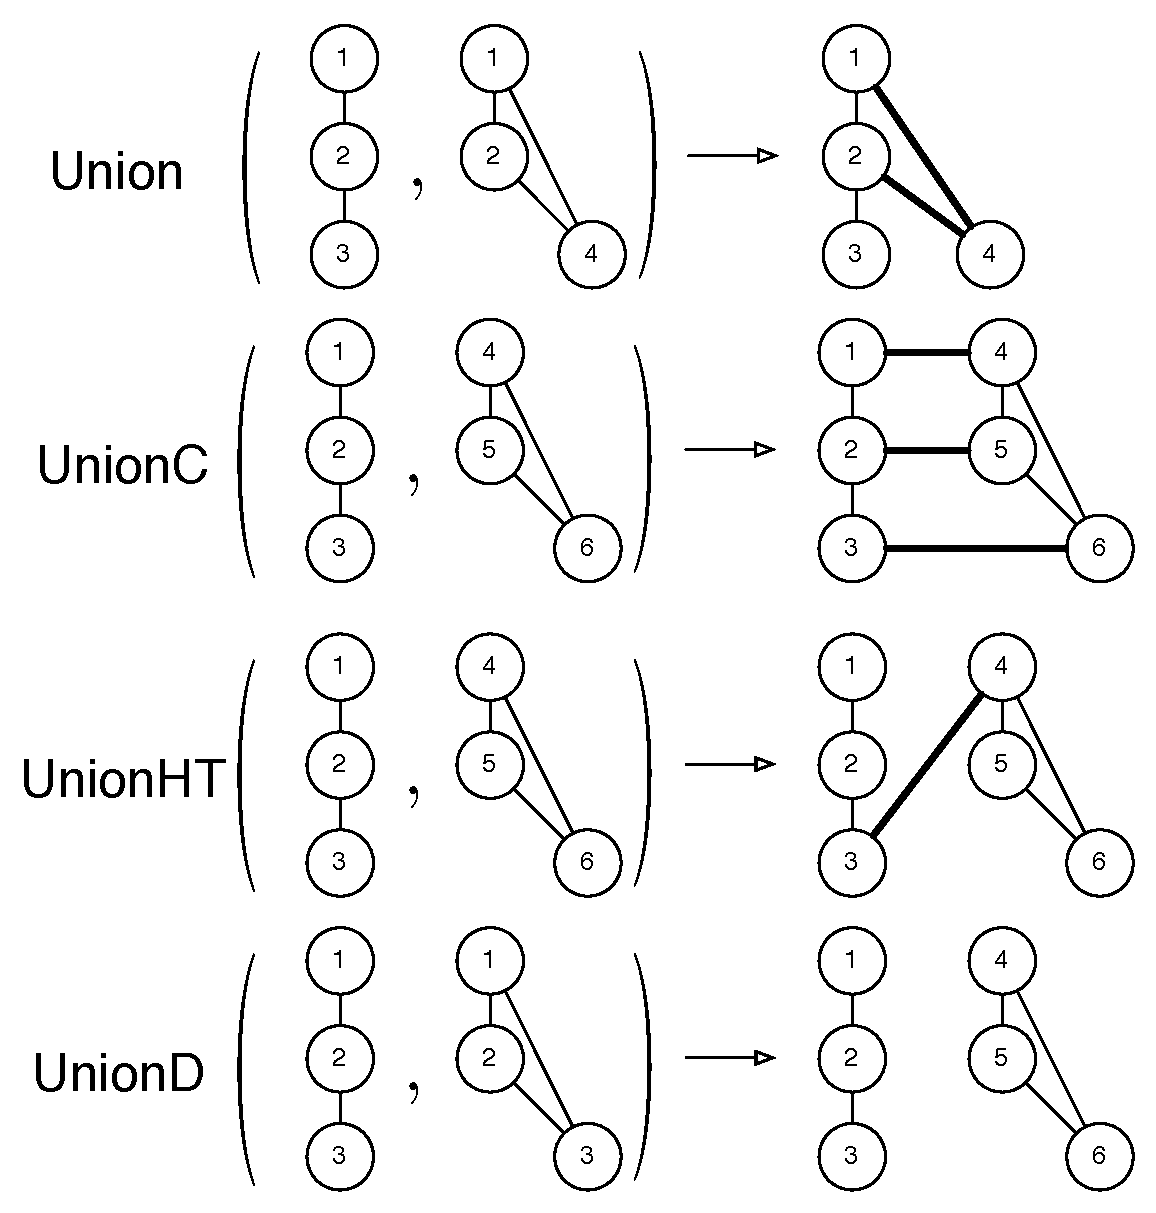
\includegraphics[width=\linewidth]{./figures/GraphCombinators.pdf}}
  \caption{test figure two}
  \label{fig:test2}\par\vfill
  % \includegraphics[width=5cm,height=4.5cm]{im
  \caption{test figure three}
  \label{fig:test3}
\end{minipage}
\end{figure}
\section{Building Towers in Blocks World}

\subsection{The Blocks World Domain}

\subsection{Learned Tower programs}

\section{Discussion}

\subsection{Relation to Prior Work}

\subsection{Limitations of SEC}


\bibliographystyle{plain}
\bibliography{eyal_bib}

\end{document}
